\section{Sets}

\begin{frame}{Set: collection of objects}
  \begin{itemize}
    \setlength\itemsep{4mm}
    \item Denoted by capital letters: $A,B,X$
    \item Objects in a set are called elements.
    \item Elements are denoted by lower case letters: $a,b,x$
    \item Curly braces around elements: $A = \{a_0,a_1,a_2\}$
  \end{itemize}
  \vspace{3mm}
  \begin{exampleblock}{Examples}
    \begin{novspace}
      \begin{flalign*}
      A &= \{ 1, 2, 3 \} \\
      B &= \{ p \mid p \ \textrm{is a prime number} \}
      \end{flalign*}
    \end{novspace}
  \end{exampleblock}
\end{frame} 
 

\begin{frame}{No order and no count}
  \begin{alertblock}{A set doesn’t maintain an order of its elements:}
      \begin{flalign*}
        & \{1,2,3\} \  = \  \{1,3,2\} \  = \  \{2,1,3\} \  = \   \{2,3,1\}\\
        & = \  \{3,1,2\} \  = \  \{3,2,1\}
      \end{flalign*}
    \end{alertblock}
    \vspace{3mm}
    \begin{alertblock}{An object is either in the set or not:}
      \begin{flalign*}
        & \{1,2,2,3\} \  = \   \{1,2,3\}
      \end{flalign*}
  \end{alertblock}
\end{frame}

\begin{frame}[fragile]{Question: is $1.0$ an element of $\mathbb{Z}$?}

  To a programmer, the answer is likely no, since $1.0$ is a floating-point number and not an integer.
  Compilers will sometimes give errors if you give $1.0$ where an integer is expected.

  \begin{minted}{python}
IPython 6.1.0 -- An enhanced Interactive Python.
Type '?' for help.
In [1]: i = 1.0
In [2]: a = [1,4,9,16]
In [3]: a[i]
TypeError: list indices must be integers or slices,
not float
In [4]: a[int(i)]
Out[4]: 4
  \end{minted}
\end{frame}

\begin{frame}[fragile]{Question: is $1.0$ an element of $\mathbb{Z}$?}
  Most mathematicians, on the other hand, will likely say $1.0$ is an integer.
  To them, $1$ and $1.0$ are just different representations of the same point on a number line.
  They think of $\mathbb{Z}$ as a subset of the real numbers $\mathbb{R}$.
  Every number on the usual number line is a real number, including $\pi$, $1.5$ and $10$.

  \begin{center}
    \includegraphics[width=0.8\textwidth]{img/numberline.png} 
  \end{center}

  There's not a lot we can do, other than to provide some context when we consider such sets.
  The discussion can get philosophical, especially in discussions about symbols and semantics.
  Again, this is an important concept in the theory of computation.
\end{frame}



\begin{frame}{Sets containing sets}
  \begin{alertblock}{Subsets}
    \setlength\itemsep{0mm}
    \belowdisplayskip=0pt
    $A$ is a subset of $B$ if all the elements of $A$ are in $B$.
    \begin{flalign*}
      A={1,2,3,4} \qquad   B={2,3} \qquad B \subset A
    \end{flalign*}
  \end{alertblock}

  \begin{alertblock}{Powersets}
    Some sets contain other sets as elements.
    The powerset of a set is the set containing all subsets of it:
    \begin{flalign*}
      A &= {1,2,3} \\
      \mathcal{P}(A) &= \{\{\},\{1\},\{2\},\{3\},\{1,2\},\{1,3\},\{2,3\},\{1,2,3\}\}
    \end{flalign*}
    Note $A$ contains 3 elements and $\mathcal{P}(A)$ contains $2^3=8$.
  \end{alertblock}
\end{frame}


\begin{frame}[fragile]{Famous sets}
  \begin{description}[123]
    \setlength\itemsep{5mm}
    \item[$\mathbb{N}$] -- the natural numbers $\{ 1, 2, 3, \ldots \}$.
    \item[$\mathbb{N}_0$] -- the natural numbers with zero $\{ 0, 1, 2, 3, \ldots \}$.
    \item[$\mathbb{Z}$] -- the integers $\{ \ldots, -2, -1, 0, 1, 2, \ldots \}$.
    \item[$\mathbb{Q}$] -- the rational numbers $\{ \frac{m}{n} \mid m, n \in \mathbb{Z} \}$.
    \item[$\mathbb{R}$] -- the \href{https://en.wikipedia.org/wiki/Real\_number\#Definition}{real numbers}.
    \item[$\mathbb{C}$] -- the complex numbers $\{ a + bi \mid a, b \in \mathbb{R}, i^2 = -1 \}$.
  \end{description}
\end{frame}


\begin{frame}[fragile]{Sizes of sets}
  \begin{topdisp}
  $$ A = \{a,b,c\} \  \Rightarrow \  \vert A \vert = 3 $$
  \end{topdisp}
  \begin{itemize}
    \setlength\itemsep{4mm}
    \item Number of elements is denoted with vertical lines.
    \item The set of all prime numbers is an \emph{infinite} set.
    \item Infinite sets can still have a notion of size.
    \item $\mathbb{R}$ \href{https://en.wikipedia.org/wiki/Cantor\%27s\_diagonal\_argument}{is bigger than} $\mathbb{N}$ even though they're both infinite -- important consequences for computation.
  \end{itemize}
\end{frame}


\begin{frame}{Operations on sets}
  \begin{topdisp}
    $$ A = \{1,2,3\} \qquad  B = \{2,3,4\}$$
  \end{topdisp}
  \vspace{4mm}
  \begin{description}[Intersection:]
    \setlength\itemsep{6mm}
    \item[Union:] $A \cup B = \{1,2,3,4\}$, in $A$ \textbf{or} $B$.
    \item[Intersection:] $A \cap B = \{2,3\}$, in $A$ \textbf{and} $B$.
    \item[Difference:] $A \setminus B = \{1\}$, in $A$ \textbf{not} $B$.
  \end{description}
\end{frame}






\section{Tuples}

\begin{frame}{Tuples: finite list of elements taken from sets}
  \begin{topdisp}
    $$t = (2,1,1) \qquad t \in \mathbb{N} \times \mathbb{N} \times \mathbb{N} \qquad |t| = 3$$
  \end{topdisp}
  \begin{itemize}
    \setlength\itemsep{2mm}
    \item Round brackets denote tuples, and $t$ is a $3$-tuple or a triple.
    \item Tuples have order, and can repeat elements.
    \item Sometimes we omit the brackets and commas: $t = 211$.
    \item $\mathbb{N} \times \mathbb{N} \times \mathbb{N}$ is sometimes shortened to $\mathbb{N}^3$.
    \item The first $\mathbb{N}$ means the first element comes from $\mathbb{N}$.
    \item The second $\mathbb{N}$ means the second element comes from $\mathbb{N}$, etc.
    \item Note that there is a single empty tuple: $()$.
  \end{itemize}
\end{frame}

\begin{frame}[fragile]{Cartesian products of sets}
  \begin{topdisp}
    $$A = \{1,2,3\} \qquad B = \{x,y\}$$
    $$A \times B = \{(1,x),(2,x),(3,x),(2,y),(2,y),(3,y)\}$$
  \end{topdisp}
  
  \begin{itemize}
    \item $A \times B$ is called the cartesian product of $A$ and $B$ -- the set of tuples with first element from $A$ and second from $B$.
    \item $\mathbb{R} \times \mathbb{R} = \mathbb{R}^2$ is the usual 2D plane where we draw plots.
    \item Can extend to any length of tuple: $\mathbb{R}^3$ is the 3D plane.
  \end{itemize}

  \begin{center}
    \resizebox{20mm}{20mm}{%
      \begin{tikzpicture}
        \begin{axis}
          \addplot[color=red]{exp(x)};
        \end{axis}
      \end{tikzpicture}
    }
    \hspace{5mm}
    \resizebox{20mm}{20mm}{%
      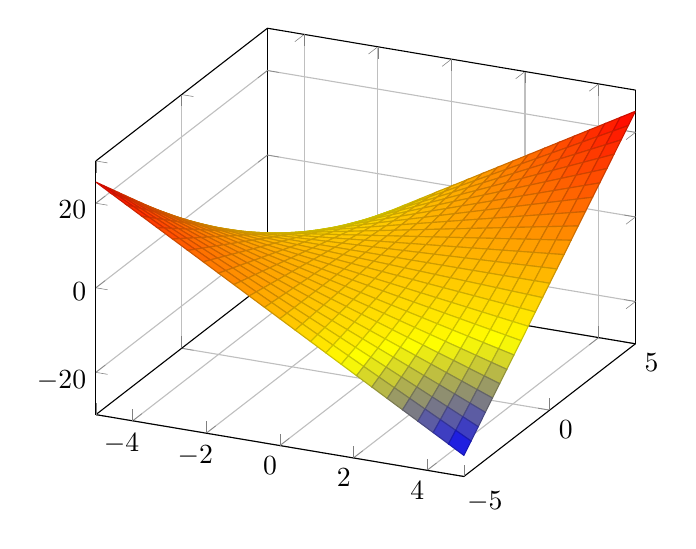
\begin{tikzpicture}
        \begin{axis}[grid=both]
          \addplot3[surf,shader=faceted] {x*y};
        \end{axis}
      \end{tikzpicture}
    }
  \end{center}
\end{frame}

\begin{frame}[fragile]{Multisets}
  \begin{topdisp}
    $$M = \{(a, 2), (b, 10), (x,5) \}$$
  \end{topdisp}
  \begin{itemize}
    \setlength\itemsep{3mm}
    \item We can use sets and tuples to define other data structures.
    \item A multiset over a set $A$ is a subset of $A \times \mathbb{N}$ such that every element of $A$ appears exactly once as the first element in a tuple.
  \end{itemize}
\end{frame}